\textbf{Breitensuche}\\
Betrachten Sie den Graphen im unten angegebenen Bild. Dort finden sich 6 Knoten mit Kanten zu anderen Knoten. Wir codieren den Graphen mit der unten angegebenen Liste von Listen.
Der nullte Eintrag der Liste enthält die Elemente 1 und 5, weil der Knoten 0 nach 1 und 5 zeigt und so weiter...\\~\\
\vspace{.5cm}
\begin{minipage}{.45\textwidth}
\begin{verbatim}
[[1, 5],
 [2,4],
 [],
 [],
 [3, 2,],
 [2]]
\end{verbatim} 
\end{minipage}
\begin{minipage}{.45\textwidth}
	\begin{center}
		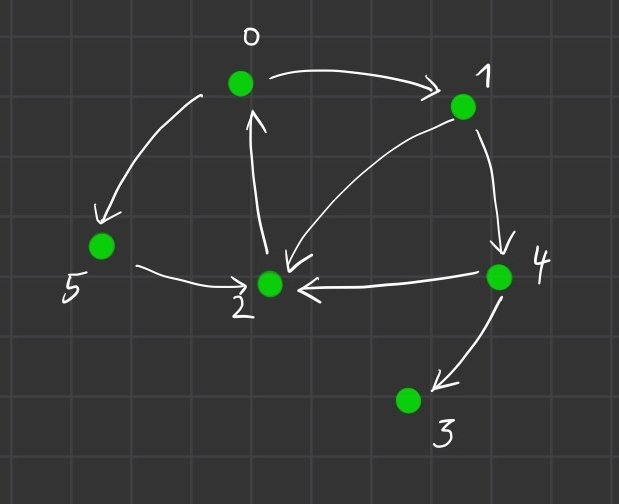
\includegraphics[scale=.2]{BreadthFirstSearch/BreadthFirstSearch.jpg}
	\end{center}
\end{minipage}


Schreiben Sie einen \href{https://de.wikipedia.org/wiki/Breitensuche}{Breitensuche-Algorithmus} in Python, der gestartet an dem Knoten 0, einen Weg zum Knoten 3 findet und stellen Sie vor wie er funktioniert.\\

\textit{Hinweis:} Arbeiten Sie mit dem Datentyp \texttt{list} und verwenden Sie die Methoden \texttt{.append(), .copy(), .pop()}.
